\let\negmedspace\undefined
\let\negthickspace\undefined
\documentclass[journal]{IEEEtran}
\usepackage[a5paper, margin=10mm, onecolumn]{geometry}
%\usepackage{lmodern} % Ensure lmodern is loaded for pdflatex
\usepackage{tfrupee} % Include tfrupee package

\setlength{\headheight}{1cm} % Set the height of the header box
\setlength{\headsep}{0mm}     % Set the distance between the header box and the top of the text

\usepackage{gvv-book}
\usepackage{gvv}
\usepackage{cite}
\usepackage{amsmath,amssymb,amsfonts,amsthm}
\usepackage{algorithmic}
\usepackage{graphicx}
\usepackage{textcomp}
\usepackage{xcolor}
\usepackage{txfonts}
\usepackage{listings}
\usepackage{enumitem}
\usepackage{mathtools}
\usepackage{gensymb}
\usepackage{comment}
\usepackage[breaklinks=true]{hyperref}
\usepackage{tkz-euclide} 
\usepackage{listings}
% \usepackage{gvv}                                        
\def\inputGnumericTable{}                                 
\usepackage[latin1]{inputenc}                                
\usepackage{color}                                            
\usepackage{array}                                            
\usepackage{longtable}                                       
\usepackage{calc}                                             
\usepackage{multirow}                                         
\usepackage{hhline}                                           
\usepackage{ifthen}                                           
\usepackage{lscape}
\usepackage{multicol}
\begin{document}

\bibliographystyle{IEEEtran}
\vspace{3cm}

\title{4.13.17}
\author{EE25BTECH11012-BEERAM MADHURI}
% \maketitle
% \newpage
% \bigskip
{\let\newpage\relax\maketitle}

\renewcommand{\thefigure}{\theenumi}
\renewcommand{\thetable}{\theenumi}
\setlength{\intextsep}{10pt} % Space between text and floats


\numberwithin{equation}{enumi}
\numberwithin{figure}{enumi}
\renewcommand{\thetable}{\theenumi}


\textbf{Question}:\\
Three distinct points $A$, $B$ and $C$ are given in the 2-dimensional coordinate plane such that the ratio of the distance of any one of them from the point $(1,0)$ to the distance from the point $(-1,0)$ is equal to $\frac{1}{3}$. Then the circumcentre of the triangle $ABC$ is at the point:
\begin{enumerate}
\begin{multicols}{4}
\item $\left(\frac{5}{4}, 0\right)$
\item $\left(\frac{5}{2}, 0\right)$
\item $\left(\frac{5}{3}, 0\right)$
\item $(0, 0)$
\end{multicols}
\end{enumerate}
\textbf{Solution:}
let $\vec{F_1}$, $\vec{F_2}$ be the vectors such that:
\begin{table}[h!]
    \centering
    \begin{tabular}[12pt]{ |c| c|}
    \hline
    \textbf{Point} & \textbf{Vector}\\ 
    \hline
    $\mathbf{v_1}$ &  $\myvec{1\\1\\1}$\\
    \hline
    $\mathbf{v_2}$ &   $\myvec{1\\-1\\1}$\\
    \hline
     $\mathbf{v_3}$ &  $\myvec{1\\1\\-1}$\\
    \hline
    \end{tabular}
    \caption{Variables used}
    \label{table 1.9.1}
\end{table}\\
Let $\vec{P}$ be any vector in the plane of $\vec{A}$,$\vec{B}$,$\vec{C}$.\\
  given,
\begin{align}
\frac{\| \vec{PF_1} \|}{\| \vec{PF_2} \|} = \frac{1}{3}\\
\frac{\sqrt{(\vec{P}-\vec{F_1})^\top (\vec{P}-\vec{F_1})}}{\sqrt{(\vec{P}-\vec{F_2})^\top (\vec{P}-\vec{F_2})}} = \frac{1}{3}
\end{align}
Squaring on both sides
\begin{align}
9 (\vec{P}-\vec{F_1})^\top (\vec{P}-\vec{F_1}) = (\vec{P}-\vec{F_2})^\top (\vec{P}-\vec{F_2})\\
9 (\vec{P^\top} \vec{P} - \vec{P^\top} \vec{F_1} - \vec{F_1^\top} \vec{P} + \vec{F_1^\top} \vec{F_1}) = \vec{P^\top} \vec{P} - \vec{P^\top} \vec{F_2} - \vec{F_2^\top} \vec{P} + \vec{F_2^\top} \vec{F_2}
\end{align}
\begin{align}
\text{as } \vec{P^\top} \vec{F_1} = \vec{F_1}^\top \vec{P} \\
\text{and } \vec{P^\top} \vec{F_2} = \vec{F_2^\top} \vec{P}
\end{align}
\begin{align}
9 (\vec{P^\top} \vec{P} - 2\vec{P^\top} \vec{F_1} + \vec{F_1^\top} \vec{F_1}) = \vec{P^\top} \vec{P} - 2\vec{P^\top} \vec{F_2} + \vec{F_2^\top} \vec{F_2}\\
8 \vec{P^\top} \vec{P} - 2\vec{P^\top} (9\vec{F_1}-\vec{F_2}) +9\vec{F_1^\top} \vec{F_1} - \vec{F_2^\top} \vec{F_2} = 0\\
\vec{P^\top} \vec{P} - \frac{1}{4} \vec{P^\top} (9\vec{F_1}-\vec{F_2}) + \frac{9}{8} \vec{F_1^\top} \vec{F_1} - \frac{1}{8} \vec{F_2^\top} \vec{F_2} = 0
\end{align}
This can be compared with general equation of circle :
\begin{align}
||\vec{P} - \vec{C}|| = r\\
\end{align}
\text{
where ,}
\text{
$\vec{P}$ = any point on the circle}\\
\text{$\vec{C}$ = Center of circle}\\
\text{
r = radius of circle}\\
\begin{align}
(\vec{P}-\vec{C})^\top(\vec{P}-\vec{C}) = r^2\\
\vec{P}^\top\vec{P} -2\vec{P}^\top\vec{C}+\vec{C}^\top\vec{C}=r^2
\end{align}
Substituting $\Vec{P}$, $\vec{F_1}$ and $\vec{F_2}$\\
Center of circle =  $\left(\frac{5}{4}, 0\right)$

Hence, the circumcenter of the triangle is $\left(\frac{5}{4}, 0\right)$
\begin{figure}[H]
    \centering
    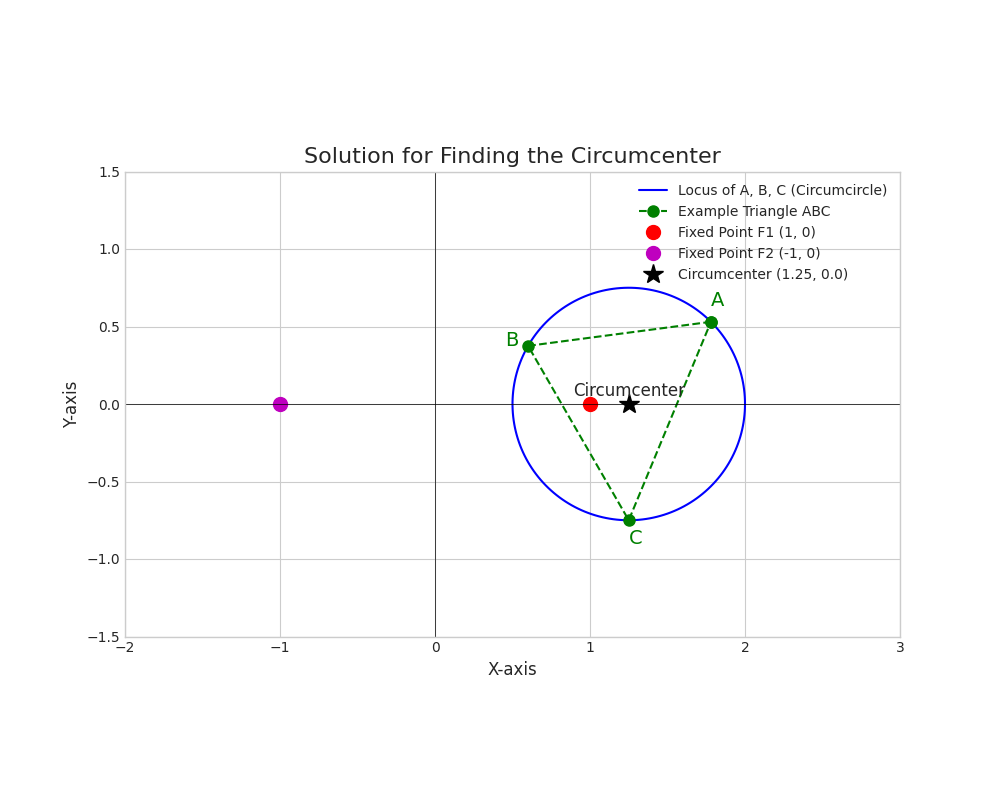
\includegraphics[width=0.85\columnwidth]{figs/graph9.png}
    \caption{4.13.17}
    \label{fig:placeholder}
\end{figure}

\end{document}